\RequirePackage[l2tabu, orthodox]{nag}
\documentclass[12pt]{article}

\usepackage{amssymb,amsmath,verbatim,graphicx,microtype,upquote,units,booktabs,hyperref,tikz,wrapfig,xcolor,pgfplots,listings,xcolor}
\usepackage[binary-units=true]{siunitx}
\usepackage[margin=10pt, font=small, labelfont=bf, labelsep=endash]{caption}

\pgfplotsset{compat=1.12}
\setcounter{secnumdepth}{2}

\title{Project \#3}
\date{Due Date: Tuesday, December 6\textsuperscript{th}, 2016}
\author{Michael Schoen, Abdirahman Osman, Illya Starikov}

\newcommand{\shellcmd}[1]{\texttt{\colorbox{gray!30}{#1}}}
\newcommand{\todo}[1]{\textbf{\colorbox{red!50}{#1}}}
\newcommand{\br}{\\\multicolumn{2}{c}{} \\ }

\begin{document}
\maketitle

For the second project, we were delighted to be able to use a higher level programming language; we\footnote{Illya.} decided to apply this new-found excitement to implement a retro game from the \num{70}s: Space Invaders.

\begin{figure}[!ht]
    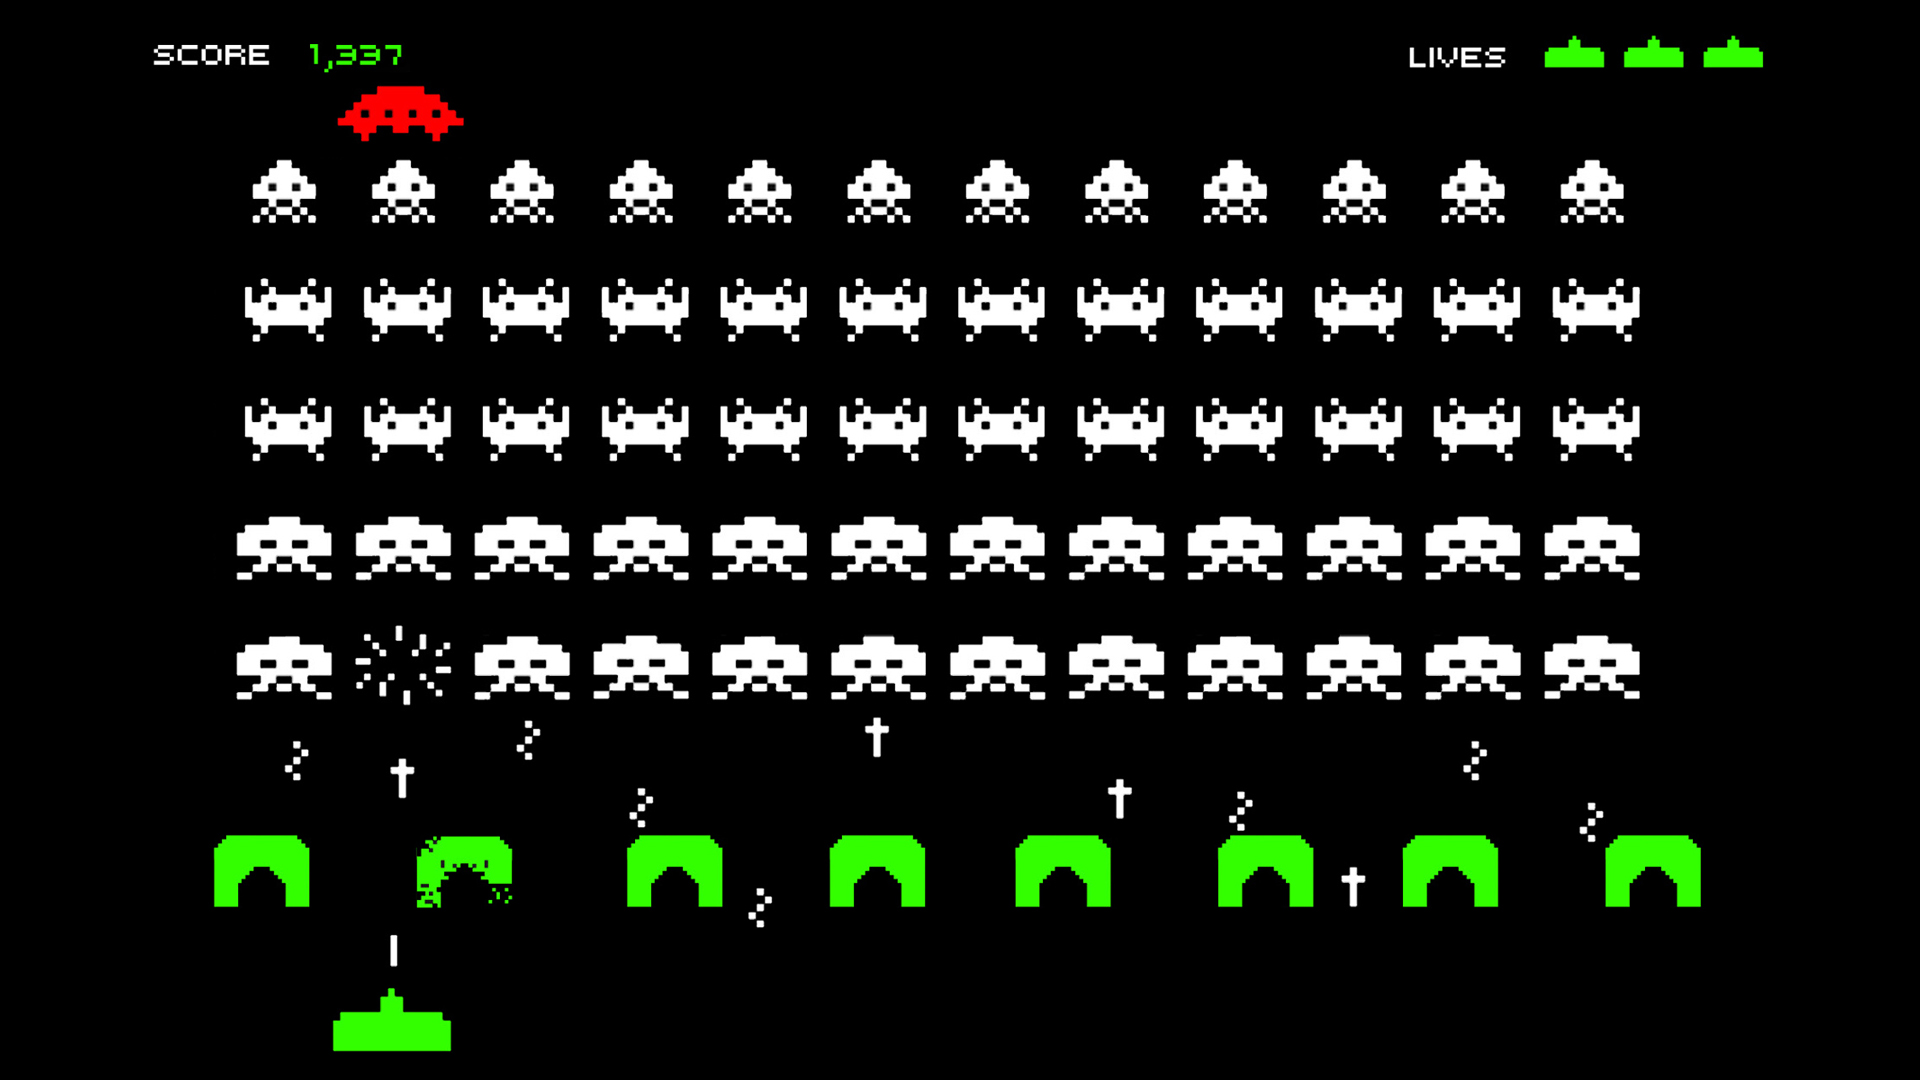
\includegraphics[width=\textwidth]{assets/space-invaders}
    \caption{The original space invaders.}
    \label{space-invaders}
\end{figure}

\section{Project Description}

\section{Problems Encountered}
Below we will list some of the ``several'' problems we ran into.

\subsection{Memory Constraints}
By far, the biggest problem we encountered was the memory constraint. The \SI{8051} has \SI{8}{\kilo\byte} of memory; our code base, with the exclusion of all the \shellcmd{malloc}s\footnote{Since \shellcmd{unsigned char} = \SI{1}{\byte}, the terminal window will roughly be $20\text{ height} \times 80\text{ width} $, we can roughly expect \SI{1.6}{\kilo\byte} to be allocated on the heap; a non-insignificant amount compared to \SI{8}{\kilo\byte}.}, it is roughly \SI{25}{\kilo\byte} --- a size a bit larger than the \num{8051} allows. Our workaround was to fight fire with fire.

Instead of ``dumbing'' our game down to get it to fit, we decided to have an external interface; specifically, a port sniffer. It would listen for input from the \num{8051}, and if there is a signal on the serial port, use that as input. If not, default to the keyboard input.

Ultimately, we were \todo{add what happened with port sniffer.}


\section{Individual Features}
\begin{itemize}
    \item Michael Schoen
    \begin{itemize}
        \item All Game Sounds
        \item Game Music
    \end{itemize}

    \item Abdirahman Osman
    \begin{itemize}
        \item Port Serialization
        \item Menu Logic
    \end{itemize}

    \item Illya Starikov
    \begin{itemize}
        \item Space Invaders Game
    \end{itemize}
\end{itemize}

\section{8051 Architecture}

\end{document}
